\chapter{Da matriz de marés às correlações entre pulsares}
\label{cap:pta}

O TG calculou a matriz de marés que uma onda massiva produziria em um
detector local e propôs, como continuação, estudar detectores esféricos
ressonantes. O Capítulo~\ref{cap:polarizacoes} mostrou que, com os
limites atuais, as assinaturas massivas só são apreciáveis em
nanohertz. Nessa banda, o detector é uma PTA, e o observável é a
correlação entre os resíduos de temporização de pares de pulsares. Este
capítulo constrói essa ponte. A Seção~\ref{sec:pta-redshift} mostra que
a resposta de temporização depende da onda apenas pela matriz de marés.
As seções seguintes calculam as correlações angulares dos setores
tensorial e de helicidade zero de Fierz--Pauli, discutem seus limites e
a degenerescência no limiar, e indicam onde a informação sobre a massa
aparece nos dados.

\section{Geometria}

Sejam $\hat p_a$ a direção da Terra para o pulsar $a$, $L_a$ sua
distância e $\hat\Omega$ a direção de propagação da onda. Para uma
componente de frequência $f$, definem-se
\begin{equation}
 \mu_a=\hat\Omega\cdot\hat p_a,\qquad
 D_a=1+\beta\mu_a,\qquad
 y_a=\frac{2\pi fL_a}{c},
 \label{eq:pta-geometria}
\end{equation}
com $\beta=\sqrt{1-(f_g/f)^2}$ como no capítulo anterior. A fase da onda
é escrita como $e^{i\omega(t-\beta\hat\Omega\cdot\mathbf x/c)}$.
Como $\beta$ é a razão entre a velocidade de grupo e $c$, a velocidade
de fase é $c/\beta>c$. O fóton emitido pelo pulsar percorre
$\mathbf x(s)=s\hat p_a$, com $t(s)=t-s/c$ e $0\le s\le L_a$; a fase da
onda no pulsar difere da fase na Terra por $e^{-iy_aD_a}$.

\section{Desvio de frequência: a resposta depende só das marés}
\label{sec:pta-redshift}

Na RG, no calibre TT, os observadores com coordenadas espaciais fixas
são geodésicos, e basta integrar a equação do fóton. Uma onda massiva
genérica tem componentes $H_{0\mu}\neq0$ que não podem ser removidas por
calibre (Capítulo~\ref{cap:polarizacoes}). Nesse caso, a Terra e o
pulsar, tratados como partículas livres, oscilam com a onda, e sua
quadrivelocidade deve ser incluída na frequência medida. Na ordem
linear, com $c=1$ e sem movimento homogêneo adicional,
\begin{equation}
 \delta u^0=-\frac{H_{00}}{2},\qquad
 \delta u^i=H_{0i}+\frac{\beta\,\Omega_i}{2}H_{00}.
 \label{eq:pta-observadores}
\end{equation}
Somando a variação do momento do fóton ao longo da trajetória e a
contração com as quadrivelocidades nos extremos, obtém-se o desvio
fracionário de frequência
\begin{equation}
 \frac{\nu_E-\nu_P}{\nu_P}
 =\frac{\hat p_a^i\hat p_a^j}{2D_a}\left(Q_{ij}^{E}-Q_{ij}^{P}\right),
 \qquad
 Q_{ij}=H_{ij}+\beta(\Omega_iH_{0j}+\Omega_jH_{0i})
 +\beta^2\Omega_i\Omega_jH_{00},
 \label{eq:pta-redshift}
\end{equation}
em que os índices $E$ e $P$ indicam avaliação na Terra, no instante de
recepção, e no pulsar, no instante de emissão. Esse tratamento dos
observadores coincide com o da revisão mais recente de Liang e Trodden
\autocite{liang2021}. A combinação $Q_{ij}$ não é arbitrária. Comparando
com a Eq.~\eqref{eq:pol-mares-geral}, verifica-se componente a
componente que
\begin{equation}
 Q_{ij}=\frac{2}{\omega^2}\,E_{ij}.
 \label{eq:pta-Q-mares}
\end{equation}
Portanto,
\begin{equation}
 \boxed{\;
 \frac{\nu_E-\nu_P}{\nu_P}
 =\frac{\hat p_a^i\hat p_a^j}{\omega^2D_a}
 \left[E_{ij}^{E}-E_{ij}^{P}\right].\;}
 \label{eq:pta-redshift-mares}
\end{equation}

Esse resultado tem uma leitura simples. A resposta de temporização a
uma onda plana, em qualquer teoria métrica e para qualquer polarização,
depende apenas da matriz de marés, que não depende do calibre. Ela é a
projeção de $E_{ij}$ sobre a linha de visada, na Terra e no pulsar,
dividida pelo fator de Doppler $D_a$. As componentes métricas
individualmente grandes da helicidade zero
(Seção~\ref{sec:pol-escala}) cancelam-se nessa combinação. O objeto que
o TG calculou para detectores locais é, assim, exatamente o que
determina a resposta de uma PTA. O resíduo de temporização é a integral
temporal do desvio de frequência; no domínio de Fourier,
$\tilde r_a(f)=\tilde z_a(f)/(i2\pi f)$.

Escrevendo $E_{ij}=\frac12\omega^2h_A\epsilon^A_{ij}$ para cada
polarização $A$, com $\epsilon^A_{ij}$ a parte espacial de
$Q_{ij}/h_A$, a resposta do pulsar $a$ a uma onda vinda de $\hat\Omega$
é proporcional a
\begin{equation}
 R_a^A=\frac{\hat p_a^i\hat p_a^j\epsilon^A_{ij}}{2}\,g(y_a,D_a),
 \qquad
 g(y,D)=\frac{1-e^{-iyD}}{D}
 =iy\,e^{-iyD/2}\sinc\!\left(\frac{yD}{2}\right).
 \label{eq:pta-resposta}
\end{equation}
Os termos $1$ e $e^{-iyD}$ são, respectivamente, os termos da Terra e do
pulsar. A forma com $\sinc x=\sin x/x$ mostra que o ponto $D=0$,
possível apenas quando $\beta=1$ e a onda se propaga do pulsar para a
Terra, é uma singularidade removível: $g(y,0)=iy$.

\section{Correlações angulares}

Para um fundo estocástico, gaussiano, isotrópico e não polarizado, com
potência $S_A(f)$ por polarização, a covariância entre os resíduos de
dois pulsares é
\begin{equation}
 S^r_{ab}(f)=\frac{1}{6\pi^2f^2}\sum_{\rm setores}S_A(f)\,\Gamma^A_{ab}(f),
 \qquad
 \Gamma^A_{ab}(f)=\mathcal N_A\int d^2\hat\Omega\;
 \sum_{A\in\text{setor}}R_a^AR_b^{A*},
 \label{eq:pta-orf}
\end{equation}
em que $\Gamma_{ab}$ é a função de correlação angular, ou ORF. Para o
setor tensorial, fixa-se $\mathcal N_T=3/(8\pi)$, de modo que, na RG e
para pulsares muito distantes, a autocorrelação é um e a correlação
entre pulsares distintos é a curva de Hellings--Downs. A mesma
normalização é mantida para todo $\beta$: renormalizar a ORF para cada
massa absorveria parte da dependência física em uma redefinição da
amplitude do sinal. A matriz $\Gamma_{ab}$ é hermitiana e positiva
semidefinida. Pulsares a distâncias diferentes podem produzir partes
imaginárias não nulas, que devem ser mantidas.

\subsection{Setor tensorial}

Somando as duas polarizações transversas com o projetor
$P_{ij}=\delta_{ij}-\Omega_i\Omega_j$, obtém-se
\begin{equation}
 \Gamma^T_{ab}=\frac{3}{32\pi}\int d^2\hat\Omega\;
 \left[2(\cos\zeta-\mu_a\mu_b)^2-(1-\mu_a^2)(1-\mu_b^2)\right]
 g(y_a,D_a)\,g^*(y_b,D_b),
 \label{eq:pta-orf-tensorial}
\end{equation}
com $\cos\zeta=\hat p_a\cdot\hat p_b$. Três limites organizam o
comportamento dessa função.

\paragraph{Termo da Terra.} Para pulsares distintos e distâncias grandes
($y\gg1$, com $\beta$ não pequeno), os termos dos pulsares oscilam
rapidamente com a direção e sua contribuição média é pequena. Resta
$g\to1/D$, e a correlação é uma função apenas de $\zeta$ e $\beta$, com
forma fechada conhecida \autocite{cordes2025,liang2021}. Em $\beta=1$,
ela é a curva de Hellings--Downs, Eq.~\eqref{eq:fund-hd}. Para
$\beta\to0$,
\begin{equation}
 \Gamma^{T,\rm Terra}(\zeta)=\frac{P_2(\cos\zeta)}{5}
 +\frac{\beta^2}{35}\left[2P_2(\cos\zeta)+P_3(\cos\zeta)\right]
 +O(\beta^4),
 \label{eq:pta-limiar-terra}
\end{equation}
isto é, no limiar a correlação é um quadrupolo puro. A
Figura~\ref{fig:pta-orf} (esquerda) mostra a transição de
Hellings--Downs para o quadrupolo à medida que $\beta$ diminui. A
correlação em pequenas separações cai de $1/2$ para $1/5$; o mínimo se
desloca para $90^\circ$ e fica mais raso.

\paragraph{Autocorrelação.} Na RG, com distância finita,
\begin{equation}
 \Gamma^{T}_{aa}=1-\frac{3}{2y^2}\left[1-\frac{\sin2y}{2y}\right],
 \label{eq:pta-auto-rg}
\end{equation}
que tende a um para $y\gg1$ \autocite{cordes2025}. Para $0<\beta<1$ e
$y\to\infty$, a autocorrelação tende a
$[6\beta-4\beta^3+3(\beta^2-1)\ln\frac{1+\beta}{1-\beta}]/(2\beta^5)$,
que vale $2/5$ quando $\beta\to0$ \autocite{cordes2025}.

\paragraph{Limiar e coerência do termo do pulsar.} Em $\beta=0$, $D=1$
para todas as direções. A fase do termo do pulsar deixa de depender da
direção, e a média angular não o elimina:
\begin{equation}
 \Gamma^T_{ab}\big|_{\beta=0}
 =\left(1-e^{-iy_a}\right)\left(1-e^{iy_b}\right)\frac{P_2(\cos\zeta)}{5},
 \qquad
 \Gamma^T_{aa}\big|_{\beta=0}=\frac45\sin^2\frac{y_a}{2}.
 \label{eq:pta-limiar-completo}
\end{equation}
A autocorrelação oscila com a distância e não tem limite para
$y\to\infty$. O limite $2/5$ citado acima pressupõe tomar $y\to\infty$
antes de $\beta\to0$, e os dois limites não comutam. A escala que
controla a incoerência dos termos dos pulsares é $\beta y$, e não $y$.
Perto do limiar, justamente onde a massa tem mais efeito, a correlação
depende das distâncias aos pulsares. A aproximação de ``apenas termo da
Terra'' deixa de ser segura e as distâncias precisam ser modeladas.

\subsection{Setor de helicidade zero de Fierz--Pauli}

Para a polarização \eqref{eq:pol-helicidade-zero}, a projeção na linha
de visada é
\begin{equation}
 \hat p^i\hat p^j\epsilon^{(0)}_{ij}
 =\frac{1+(2\beta^2-3)\mu^2}{\sqrt3}
 \equiv\frac{A_\beta(\mu)}{\sqrt3},
 \label{eq:pta-projecao-escalar}
\end{equation}
e, com a mesma convenção por estado usada no setor tensorial,
\begin{equation}
 \Gamma^{0}_{ab}=\frac{1}{32\pi}\int d^2\hat\Omega\;
 A_\beta(\mu_a)A_\beta(\mu_b)\,g(y_a,D_a)\,g^*(y_b,D_b).
 \label{eq:pta-orf-escalar}
\end{equation}
A função $A_\beta(\mu)$ mistura a resposta \emph{breathing}, proporcional
a $1-\mu^2$, e a longitudinal, proporcional a $\mu^2$, com o peso fixado
pelo vínculo \eqref{eq:pol-vinculo-escalar}. A mistura tem uma
consequência prática. Se a resposta for escrita como
$A_\beta=b(\mu)+l(\mu)$, a correlação contém, além de $\Gamma_{bb}$ e
$\Gamma_{ll}$, os termos cruzados $\Gamma_{bl}+\Gamma_{lb}$. Tratar
\emph{breathing} e longitudinal como setores independentes, como é usual
em buscas fenomenológicas, descarta esses termos e descreve outra
teoria. O efeito não é pequeno. No limiar, para pulsares a $90^\circ$ e
apenas o termo da Terra, a correlação vinculada vale $-1/20$; sem os
termos cruzados, ela seria $\Gamma_{bb}+\Gamma_{ll}=1/20+1/30=+1/12$.
O sinal muda.

Os limites da Eq.~\eqref{eq:pta-orf-escalar} para o termo da Terra são
\begin{equation}
 \Gamma^{0,\rm Terra}\big|_{\beta=0}=\frac{P_2(\cos\zeta)}{10},
 \qquad
 \Gamma^{0,\rm Terra}\big|_{\beta\to1}=\frac{3+\cos\zeta}{24}.
 \label{eq:pta-limites-escalar}
\end{equation}
O segundo é a forma conhecida da correlação de um modo \emph{breathing}
puro \autocite{lee2008}. Isso é consistente com a conclusão da
Seção~\ref{sec:pol-escala}: longe do limiar, a helicidade zero de
Fierz--Pauli se comporta como um modo escalar transversal. Esse limite é
formal, porque as componentes métricas de $\epsilon^{(0)}$ crescem como
$1/\chi$ e o regime linear exige amplitudes correspondentemente
pequenas. A Figura~\ref{fig:pta-orf} (direita) mostra a transição entre
os dois limites.

\begin{figure}[htbp]
 \centering
 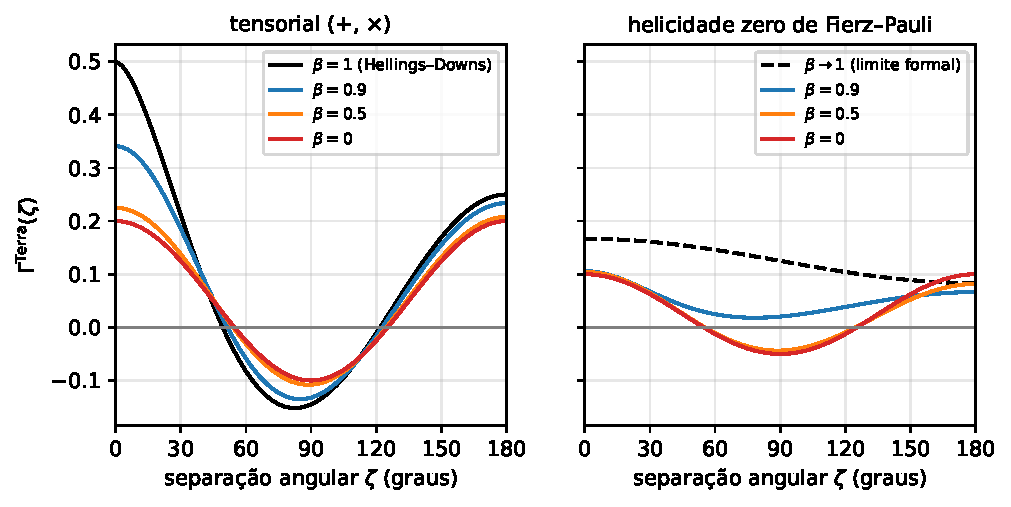
\includegraphics[width=\textwidth]{../figuras/orf_terra.pdf}
 \caption{Correlações angulares (apenas termo da Terra) para
 diferentes razões de velocidade $\beta=\sqrt{1-(f_g/f)^2}$. Esquerda:
 setor tensorial, de Hellings--Downs ($\beta=1$) ao quadrupolo
 $P_2/5$ ($\beta=0$). Direita: helicidade zero de Fierz--Pauli, do
 \emph{breathing} $(3+\cos\zeta)/24$ ($\beta\to1$) ao quadrupolo
 $P_2/10$ ($\beta=0$). Curvas calculadas por integração direta sobre a
 esfera e conferidas contra as formas fechadas e os limites
 analíticos.}
 \label{fig:pta-orf}
\end{figure}

\section{A degenerescência no limiar e sua origem}
\label{sec:pta-degenerescencia}

As Eqs.~\eqref{eq:pta-limiar-terra} e \eqref{eq:pta-limites-escalar}
mostram que, no limiar, $\Gamma^0=\Gamma^T/2$. O mesmo vale para a
correlação completa com termos dos pulsares, pois, com $D=1$, o fator
$g$ é idêntico nos dois setores. Como o setor tensorial soma dois
estados e o escalar tem um, a igualdade significa que \emph{cada estado
de polarização produz a mesma correlação angular}. A covariância dos
resíduos depende então apenas da soma das potências de todos os estados,
$2S_T+S_0$, em que $S_T$ é a potência por polarização tensorial.
Em uma única frequência no limiar, a forma angular não distingue
tensor de escalar.

A razão é a simetria discutida na Seção~\ref{sec:pol-grupo}. No limiar, a onda é
homogênea, e os estados de Fierz--Pauli são as componentes de um tensor
de marés espacial, simétrico e sem traço
($p_l=-p_b$ para a helicidade zero). A média sobre as direções de
propagação de um fundo isotrópico, aplicada à maré de um estado de norma
fixa, só pode produzir a única estrutura invariante por rotações para
tensores sem traço,
$\propto\delta_{ik}\delta_{jl}+\delta_{il}\delta_{jk}-\frac23\delta_{ij}\delta_{kl}$.
Essa estrutura não depende do estado de partida. Projetada nas linhas de
visada, ela dá o quadrupolo $P_2(\cos\zeta)$ com o mesmo coeficiente
para todos os estados. Pelo mesmo argumento, os modos vetoriais de
Fierz--Pauli, não calculados aqui, também devem ter a mesma correlação
por estado no limiar.

A degenerescência é exata apenas em $f=f_g$. Em uma banda de
frequências, os canais acima do limiar têm $\beta>0$, e as formas
tensorial e escalar se separam (Figura~\ref{fig:pta-orf}). A capacidade
de distinguir os dois setores depende, portanto, de quantos canais estão
suficientemente acima de $f_g$ e da sensibilidade neles.

\section{Uma discrepância na literatura}

A correlação de helicidade zero foi comparada com a expansão da
equação~(45) da revisão v3 de Liang e Trodden \autocite{liang2021}. A
leitura literal de um dos termos dessa expansão, com fator angular
$\sin\xi$, dá $0{,}03162079$ para $\beta=0{,}9$ e $\xi=\pi/2$ (apenas
termo da Terra). Quatro cálculos independentes dão $0{,}02036600$: a
construção pelos observadores da Eq.~\eqref{eq:pta-redshift}, a expansão
harmônica, uma referência terrestre independente e a integração direta
usada na Figura~\ref{fig:pta-orf}. Os cálculos concordam se o fator for
$\sin2\xi$. Registra-se a discrepância na expressão examinada. Não se
afirma que ela afete os resultados numéricos daquele trabalho, que não
foram reproduzidos.

\section{Cálculo numérico e validação}

A correlação completa, com termos dos pulsares, foi calculada por duas
rotas independentes. A primeira é a quadratura direta da
Eq.~\eqref{eq:pta-orf-tensorial}, com Gauss--Legendre em $\cos\theta$ e
regra periódica no azimute. A segunda é uma expansão em funções
associadas de Legendre. Os coeficientes de cada pulsar,
\begin{equation}
 c_\ell(\beta,y)=\int_{-1}^{1}dx\,(1-x^2)^2P_\ell''(x)\,g(y,1+\beta x),
 \label{eq:pta-cl}
\end{equation}
são calculados uma vez por frequência. A ORF tensorial é
\begin{equation}
 \Gamma^T_{ab}=\frac{3}{32}\sum_{\ell\ge2}
 \frac{(2\ell+1)\,c_\ell(\beta,y_a)\,c_\ell^*(\beta,y_b)}
 {(\ell-1)\ell(\ell+1)(\ell+2)}\,P_\ell(\cos\zeta),
 \label{eq:pta-serie}
\end{equation}
que reproduz as expressões de Cordes e colaboradores para distâncias
iguais \autocite{cordes2025}. A série escalar é análoga e começa em
$\ell=0$. Um corte $\ell_{\max}$ comum a todos os pares preserva a
positividade da matriz de covariância.

As duas rotas concordaram, em 58 configurações de teste, com diferenças
máximas entre $10^{-13}$ e $5\times10^{-12}$. Essas configurações
incluem $fL/c$ de $0{,}125$ a $1000$, $\beta$ de zero a um, pares quase
coincidentes e os zeros de Hellings--Downs. O número de multipolos
necessário cresce com $\beta y$. Com resolução insuficiente, os
resultados são plausíveis, mas errados. Por exemplo, para a
autocorrelação da RG em $fL/c\simeq1000$, uma série truncada em
$\ell_{\max}=200$ dá $0{,}50$, enquanto o valor exato é
$0{,}99999996$; a convergência exigiu $\ell_{\max}\approx6400$. Por isso,
todas as configurações foram aceitas somente após refinamento separado
da quadratura e do corte multipolar. Os detalhes estão no
Apêndice~\ref{ap:reproducao}.

\section{Onde está a informação sobre a massa}
\label{sec:pta-informacao}

Com observações de duração $T$, os canais de frequência são
$f_k=k/T$. Com a massa adimensional $u=f_gT$, a razão de velocidade no
canal $k$ é $\beta_k=\sqrt{1-(u/k)^2}$. Dois mecanismos transportam
informação sobre a massa.

\paragraph{Suporte cinemático.} Canais com $f_k<f_g$ não contêm ondas
viajantes. Se um sinal comum é detectado no canal mais baixo, isso
implica $f_g<1/T$ quase independentemente da forma da correlação. O
limite superior resultante, $m_gc^2\lesssim h/T$, vem sobretudo do
espectro e do suporte, e não da forma angular. É consistente com o
resultado de Wu e colaboradores, segundo o qual as correlações do
NANOGrav sozinhas não limitam a massa na faixa relevante
\autocite{wu2024}.

\paragraph{Distorção da correlação.} Para $u\ll k$,
\begin{equation}
 \Gamma_{ab}(\beta_k)=\Gamma_{ab}(1)
 -\frac{u^2}{2k^2}\,\partial_\beta\Gamma_{ab}\big|_{\beta=1}
 +O(u^4).
 \label{eq:pta-fraca}
\end{equation}
A distorção cai como $1/k^2$: praticamente toda a informação angular
sobre a massa está nos primeiros canais. São justamente os canais com
menor número de ciclos observados e maior ruído vermelho.

Essa expansão também quantifica uma aproximação usada na literatura: a
avaliação da resposta em uma única frequência de referência,
$f_{\rm ref}=1/T$, aplicada a correlações comprimidas em frequência
\autocite{zhao2026}. Substituir $\beta_k$ por $\beta_1$ em todos os
canais introduz o erro
\begin{equation}
 \Gamma_{ab}(\beta_1)-\Gamma_{ab}(\beta_k)
 =-\frac{u^2}{2}\left(1-\frac{1}{k^2}\right)
 \partial_\beta\Gamma_{ab}\big|_{\beta=1}+O(u^4),
 \label{eq:pta-fref}
\end{equation}
ou seja, exagera a dispersão nos canais mais altos. Se, além disso, as
fases dos termos dos pulsares também forem avaliadas em $f_{\rm ref}$, a
aproximação passa a errar mesmo com massa nula, porque esses termos
dependem da frequência independentemente da massa. Perto do limiar, esse
segundo erro é o maior. Em um mapa das distribuições previstas para os
dados (Capítulo~\ref{cap:simulacoes}), no canto de sinal mais intenso,
o congelamento das fases chegou a uma divergência de Kullback--Leibler
de $1{,}4$~nat, e o congelamento conjunto de $\beta$ e das fases, a
$3{,}4$~nat. Se esses erros
afetam uma inferência real depende de quanta informação os dados contêm.
Essa é a pergunta do próximo capítulo.
